% !TEX root = main.tex
\section{実験}
\subsection{第1週:ダイオードの電気特性測定}

\subsubsection*{実験方法}

本実験では,ダイオードの電流-電圧特性を測定することで,その整流特性や理想係数,直列抵抗,並列抵抗などのパラメータを導出することを目的とする.

使用機器は直流電圧・電流源/モニタである \textbf{6242} を用いた.本機器は電圧を掃引しながら電流を測定する機能を有し,高精度なIV特性の測定が可能である.

\vspace{1em}
測定にあたって設定したパラメータを以下に示す.

\begin{itemize}
    \item スイープモード:DC
    \item スタート電圧:$2~\mathrm{V}$
    \item ストップ電圧:$-2~\mathrm{V}$
    \item ステップ電圧:$0.005~\mathrm{V}$
    \item 電流リミッタ:$0.002~\mathrm{A}$
    \item 測定モード:2端子測定
    \item インターフェース:USB
\end{itemize}

測定は $2~\mathrm{V}$ から $-2~\mathrm{V}$ の範囲で,$0.005~\mathrm{V}$ 間隔のスイープを行い,その際の電流値を測定した.測定されたデータはCSV形式で保存され,後の解析で用いた.

本実験の測定方式は「2端子測定」としており,ダイオードに流れる電流と印加電圧を直接取得する構成となっている.また,オート・ゼロ機能はOFFとし,メモリ・ストアはノーマル設定で使用した.

\begin{figure}[H]
    \centering
    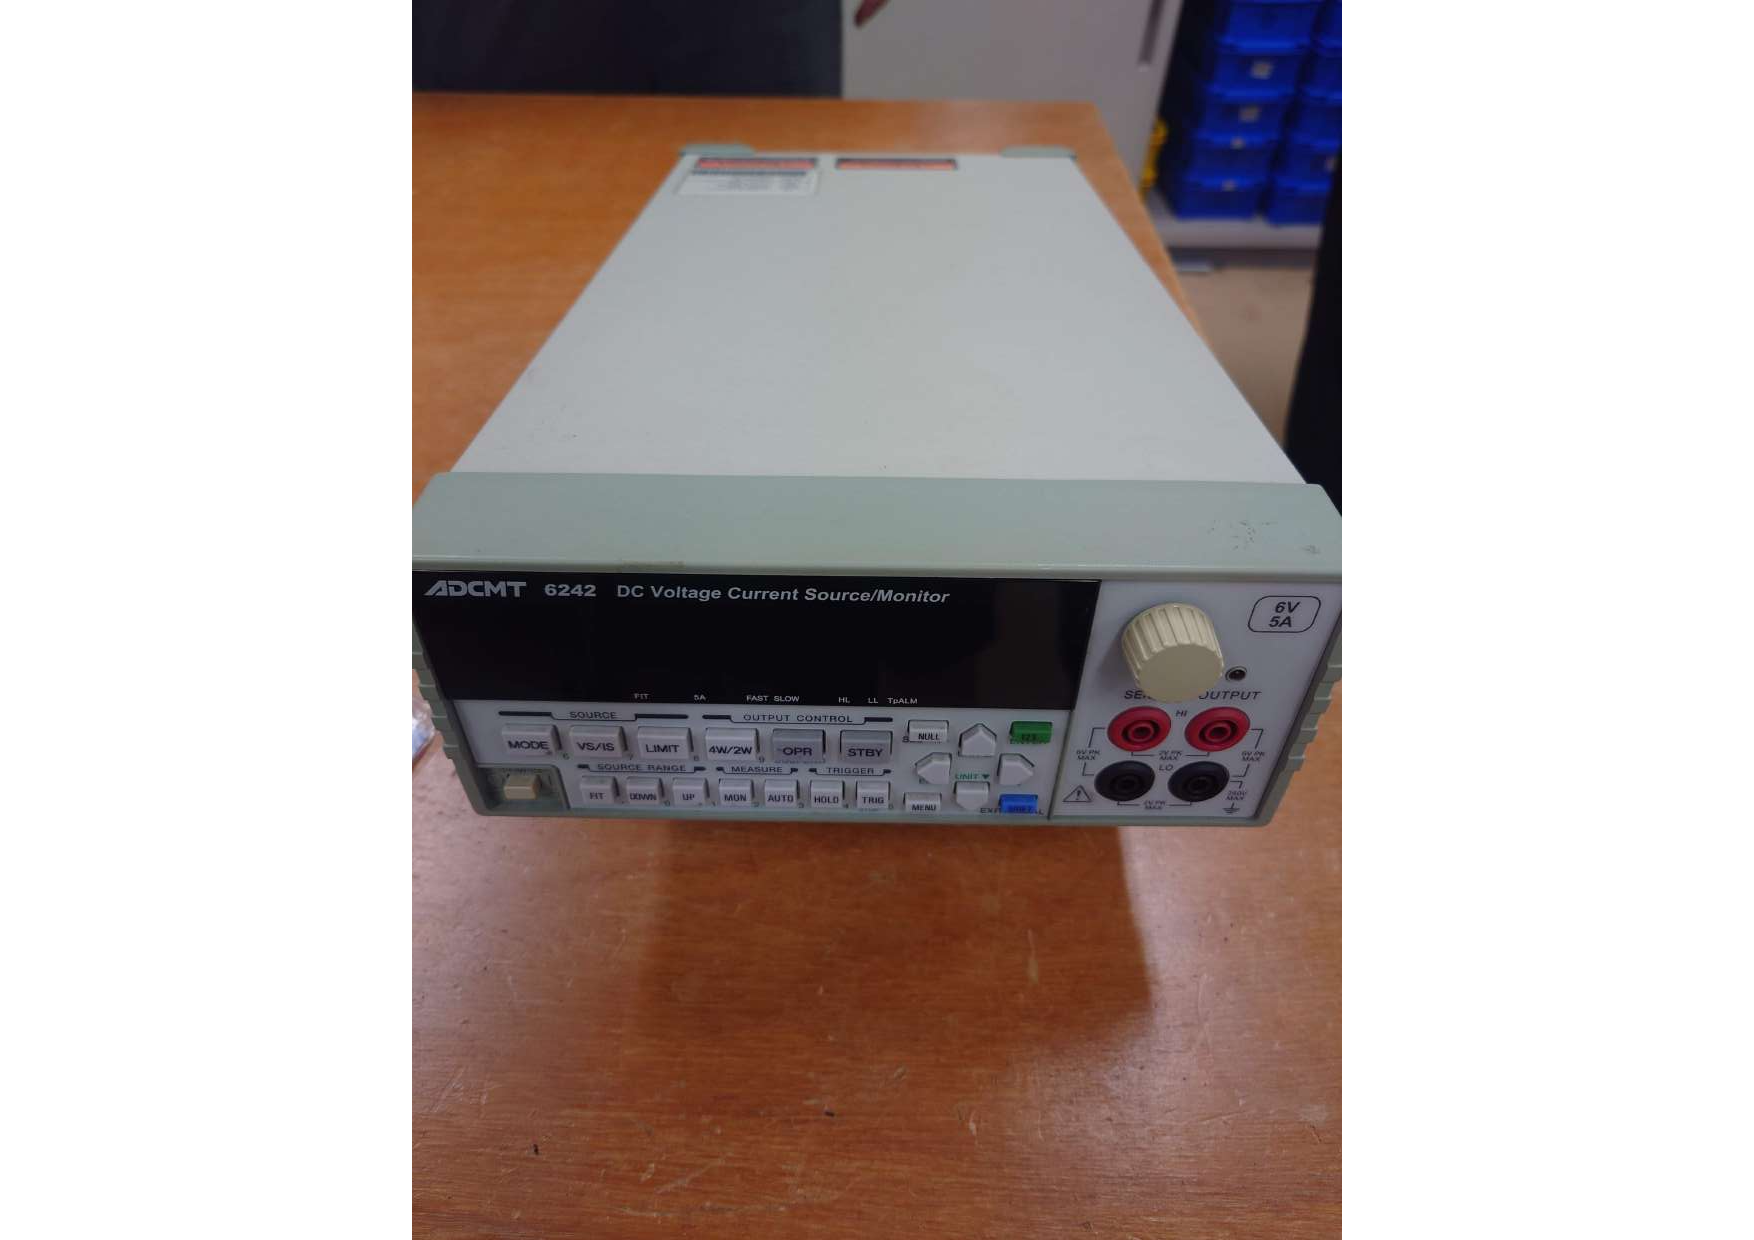
\includegraphics[width=0.6\textwidth]{figure/20250714_154436.pdf}
    \caption{測定器具6242}
    \label{fig:vig_param}
\end{figure}

\subsubsection*{パラメータ導出の理論とプログラムの仕組み}

本実験では,測定したダイオードの電圧-電流データ(CSV形式)を用いて,以下のパラメータをPythonで解析した:

\begin{itemize}
    \item 並列抵抗 \( R_p \)
    \item 直列抵抗 \( R_s \)
    \item 理想係数 \( n \)
\end{itemize}

使用プログラムは\texttt{pandas},\texttt{numpy},\texttt{scipy.stats.linregress} を用いて線形回帰を実施している.

\vspace{1em}
\paragraph{(1) 並列抵抗 \( R_p \)}

並列抵抗は,逆バイアス領域(本実験では \( V < -0.1~\mathrm{V} \))におけるI-V特性の傾きとして次のように定義される:
\begin{equation}
    R_p = \left| \frac{dV}{dI} \right|_{V < 0}
\end{equation}
この領域では,ダイオードは抵抗的に振る舞うため,\texttt{linregress} によって取得された直線の傾き(電圧 vs 電流)から \( R_p \) を導出する.

\vspace{1em}
\paragraph{(2) 直列抵抗 \( R_s \)}

順方向バイアス領域における高電流部分(例:\( 0.25~\mathrm{V} < V < 0.35~\mathrm{V} \))では,指数関数的な立ち上がりが飽和し,内部抵抗が支配的となる.この領域のI-V直線部分の傾きを用いて次のように求める:
\begin{equation}
    R_s = \frac{dV}{dI}
\end{equation}
この傾きは,ダイオード内部の接触抵抗やリード線の抵抗などの影響を含むものである.

\vspace{1em}
\paragraph{(3) 理想係数 \( n \)}

理想係数 \( n \) は,順方向バイアス領域の指数関数的なI-V関係:
\begin{equation}
    I = I_s \exp\left( \frac{qV}{nkT} \right)
\end{equation}
の両辺を自然対数変換し,直線化された関係式から導出する:
\begin{equation}
    \ln I = \ln I_s + \frac{qV}{nkT}
\end{equation}
このとき,\( \ln I \) と \( V \) の散布図を作成し,線形回帰によって傾きを求めることで,理想係数 \( n \) は以下の式で算出できる:
\begin{equation}
    n = \frac{q}{kT \cdot \text{slope}}
\end{equation}

\vspace{1em}
\paragraph{(4) 実装上の工夫と補足}

\begin{itemize}
    \item \textbf{逆方向領域}($V < -0.1$~V)で \( R_p \) を計算.ノイズを避けるために傾きが正の領域のみを対象とする.
    \item \textbf{直線領域}(例:$0.25$~V〜$0.35$~V)を用いて \( R_s \) を導出.電流がリミッタに達していない領域のみを使用.
    \item \textbf{理想係数 \( n \)} は、$\ln(I)$ と $V$ の回帰から求めるほか,複数電圧範囲での推移を可視化して,定性的評価も実施.
    \item 単位はmAで扱い,\texttt{np.log(I × 1000)} により変換を行っている.
    \item 測定ノイズや異常値を避けるため,スロープが負または異常に大きい場合(例:$n > 10$)は無視する.
\end{itemize}

\vspace{1em}
\paragraph{(5) 結果出力例}

プログラムは最終的に以下のような出力を行う:

\begin{verbatim}
=== ダイオード解析結果(1回目測定) ===
並列抵抗 Rp = 4567.89 Ω
直列抵抗 Rs = 12.34 Ω
理想係数 n  = 1.58

=== 理想係数 n の計算結果 ===
電圧 0.18 V: n = 2.01
電圧 0.23 V: n = 1.67
電圧 0.28 V: n = 1.45
\end{verbatim}

これにより,各パラメータが明確に数値化され,ダイオード特性の比較・評価が可能となる.

\subsubsection*{結果}

本実験では,2種類のショットキーダイオードを用いて特性の違いを比較した.使用した素子は以下の通りである:

\begin{itemize}
    \item \textbf{SBM1045VSS}(電力用ショットキーダイオード,最大定格:45V 10A)
    \item \textbf{1SS106}(小信号用ショットキーバリアダイオード)
\end{itemize}

両素子ともに,金属-半導体接触によるショットキー接合を用いた整流素子であり,高速応答性および低順方向電圧降下を特徴とする.

測定範囲は共通して以下のように設定した:

\begin{itemize}
    \item 電圧範囲:$-2.00~\mathrm{V} \sim 2.00~\mathrm{V}$
    \item 電流範囲(SBM1045VSS):$-3.59 \times 10^{-8}~\mathrm{A} \sim 2.00 \times 10^{-3}~\mathrm{A}$
    \item 電流範囲(1SS106):$-2.00 \times 10^{-10}~\mathrm{A} \sim 2.00 \times 10^{-3}~\mathrm{A}$
\end{itemize}

図\ref{fig:iv_log_plot}および図\ref{fig:iv_small}に,各素子のI-V特性および$\ln(I)$-$V$特性を示す.

\begin{figure}[H]
    \centering
    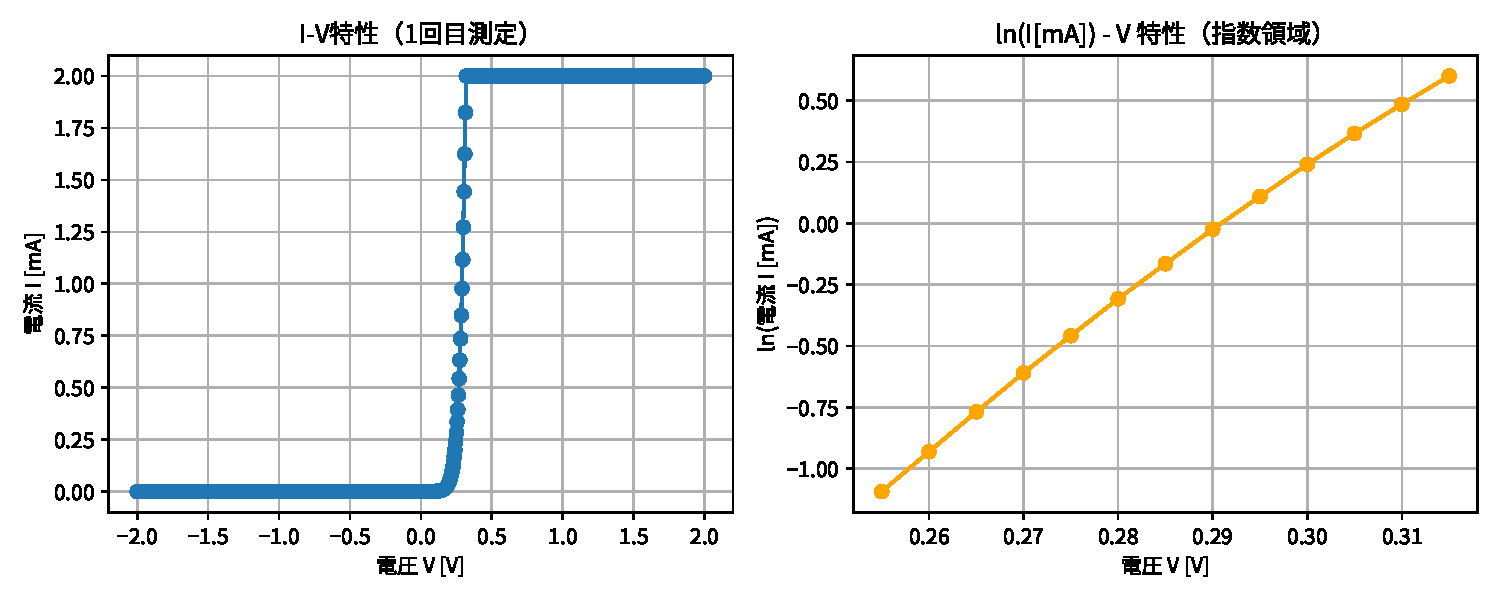
\includegraphics[width=0.8\textwidth]{figure/Figure_1.pdf}
    \caption{SBM1045VSSのI-V特性および$\ln(I)$-$V$特性}
    \label{fig:iv_log_plot}
\end{figure}

\begin{figure}[H]
    \centering
    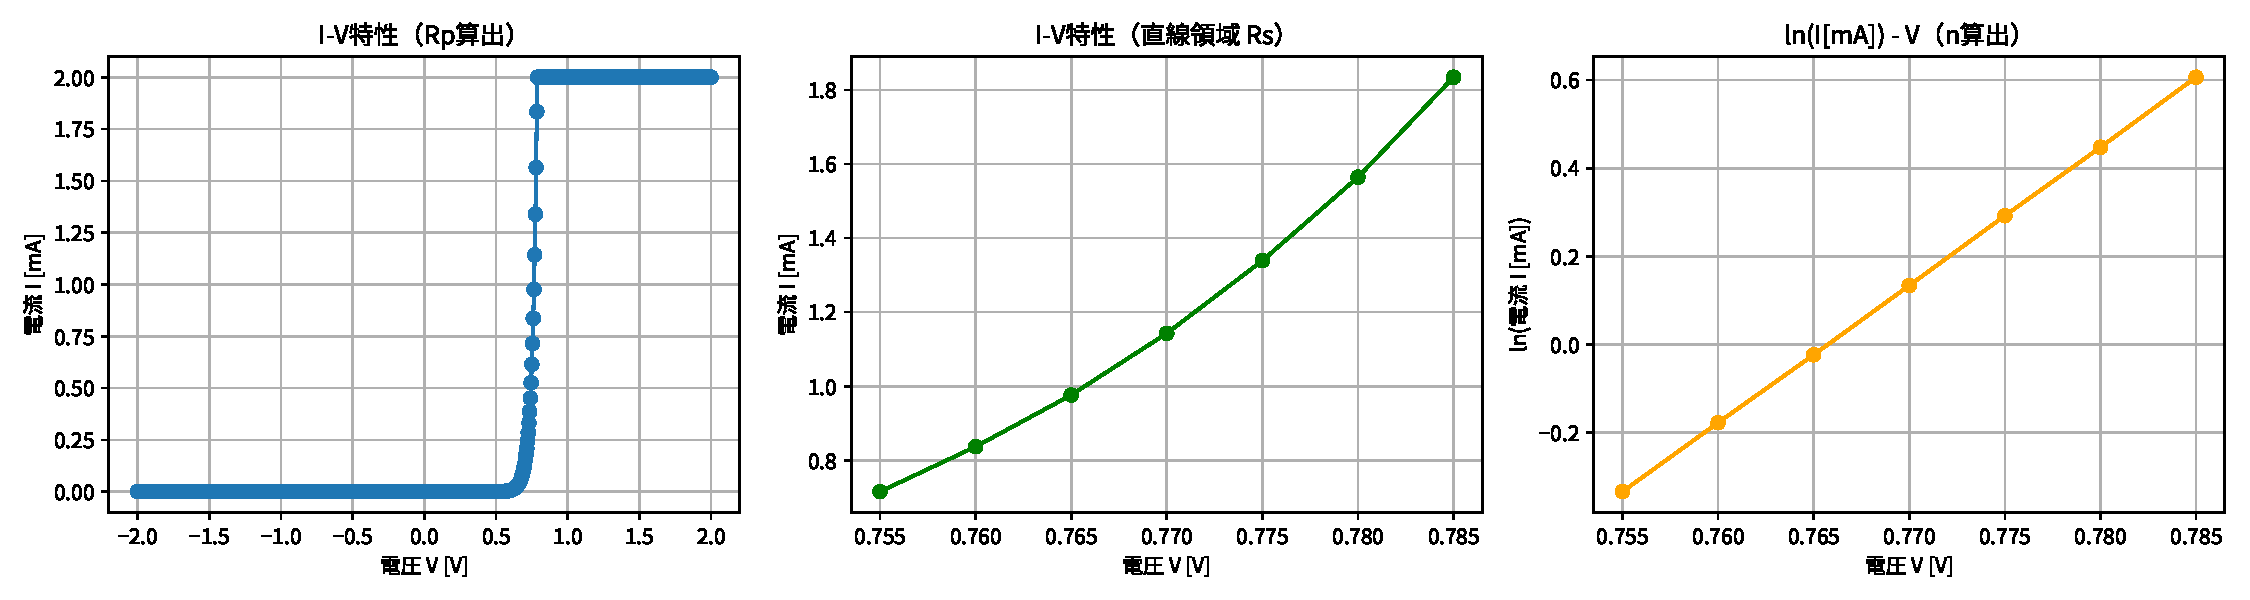
\includegraphics[width=0.8\textwidth]{figure/Figure_3.pdf}
    \caption{1SS106のI-V特性および$\ln(I)$-$V$特性}
    \label{fig:iv_small}
\end{figure}

解析により得られたパラメータを以下にまとめる:

\begin{table}[H]
    \centering
    \caption{2種ショットキーダイオードの解析結果比較}
    \begin{tabular}{lcc}
        \hline
        項目 & SBM1045VSS & 1SS106 \\
        \hline
        並列抵抗 \( R_p \) [\(\Omega\)] & \( 1.69 \times 10^8 \) & \( 1.09 \times 10^8 \) \\
        直列抵抗 \( R_s \) [\(\Omega\)] & 39.45 & 26.55 \\
        理想係数 \( n \) & 1.37 & 1.23 \\
        \hline
    \end{tabular}
\end{table}

指数領域における理想係数 \( n \) の電圧依存性を図\ref{fig:n_vs_v}および図\ref{fig:n_small}に示す.

\begin{figure}[H]
    \centering
    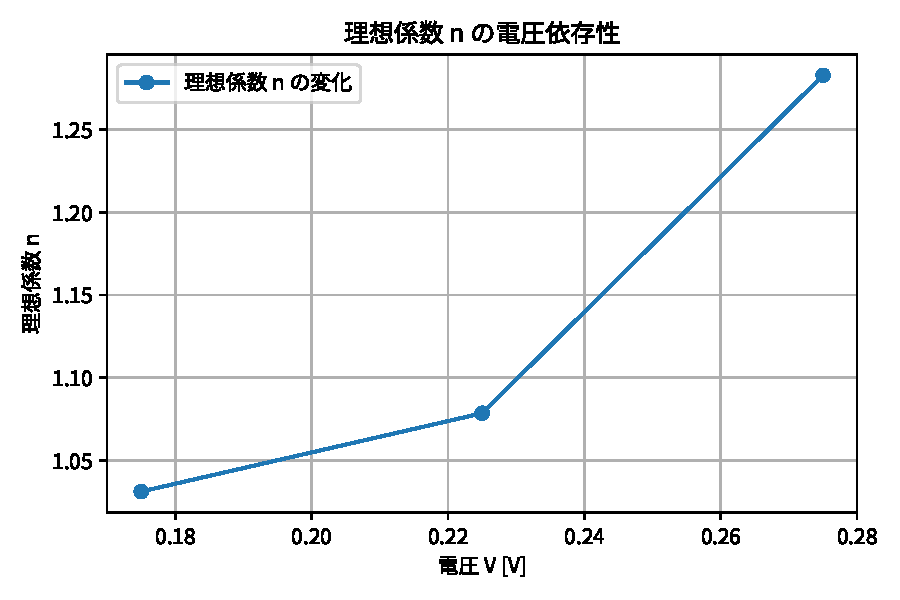
\includegraphics[width=0.6\textwidth]{figure/Figure_2.pdf}
    \caption{SBM1045VSSの理想係数 \( n \) の電圧依存性}
    \label{fig:n_vs_v}
\end{figure}

\begin{figure}[H]
    \centering
    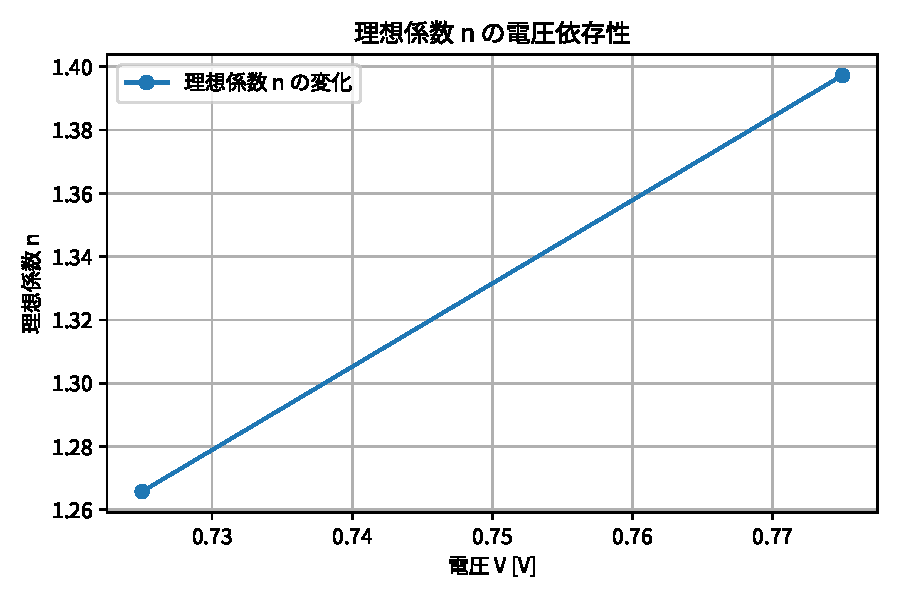
\includegraphics[width=0.6\textwidth]{figure/Figure_4.pdf}
    \caption{1SS106の理想係数 \( n \) の電圧依存性}
    \label{fig:n_small}
\end{figure}

電圧範囲別の理想係数は以下の通りである:

\begin{itemize}
    \item SBM1045VSS:
    \begin{itemize}
        \item \( V = 0.17~\mathrm{V} \):\( n = 1.03 \)
        \item \( V = 0.23~\mathrm{V} \):\( n = 1.08 \)
        \item \( V = 0.28~\mathrm{V} \):\( n = 1.28 \)
    \end{itemize}
    \item 1SS106:
    \begin{itemize}
        \item \( V = 0.73~\mathrm{V} \):\( n = 1.34 \)
        \item \( V = 0.75~\mathrm{V} \):\( n = 1.32 \)
        \item \( V = 0.77~\mathrm{V} \):\( n = 1.29 \)
    \end{itemize}
\end{itemize}

\vspace{1em}
\subsubsection*{考察}

SBM1045VSSは高電流向けのパワーショットキーダイオードであり,最大10Aの大電流に対応している.一方,1SS106は小信号用で,通信や高速スイッチング用途を意識した設計となっている.

両者とも整流特性を備えているが,以下のような違いが観察された.

\begin{itemize}
    \item \textbf{逆方向特性}:両素子とも逆方向でのリーク電流が非常に小さく,高い並列抵抗 \( R_p \) を示した.とくにSBM1045VSSは \( 1.69 \times 10^8~\Omega \) と最も高い値を示し,接合面の品質が良好であることが分かる.

    \item \textbf{順方向導通性}:1SS106の直列抵抗 \( R_s = 26.55~\Omega \) は,SBM1045VSSよりも低く,小信号用途における効率的な導通特性があることを示す.

    \item \textbf{理想係数 \( n \)}:両素子とも \( 1.0 < n < 1.5 \) の範囲内にあり,ショットキー接合として理想的な指数的増加を示している.特にSBM1045VSSの低電圧領域では \( n \approx 1.03 \) を示し,非常に理想的な指数応答が確認された.
\end{itemize}

それぞれの特性は素子の設計思想に合致しており,SBM1045VSSは電源やパワー系統で,1SS106は高速通信・スイッチング用途で真価を発揮する構造であると考えられる.
